

%  \setchapterpreamble[u]{\margintoc}
\pagelayout{wide} % No margins


\chapter*{Introduction\;}
\labch{intro}
\textbf{LLM generated slop}
\textit{give historical context on how automobiles came to be and used and how gas stations infrastacturue had to be created. And how EV chargers are very similar to the spread of ICE vehicles.}


The invention of the automobile in the late 19th century revolutionized human mobility, enabling unprecedented freedom to traverse long distances. However, this breakthrough hinged not only on the internal combustion engine (ICE) itself but also on the parallel development of a critical support system: gasoline stations. Just as early motorists relied on scattered fuel depots to power their journeys, the rise of ICE vehicles necessitated a standardized, accessible network of refueling infrastructure to sustain their adoption. This symbiotic relationship between vehicles and their energy infrastructure became a cornerstone of modern transportation, shaping urban planning, economic systems, and global energy policies.

Today, as societies pivot toward sustainability, \acrfull{EV} are heralding a similar paradigm shift. Yet their widespread adoption faces a challenge mirroring the early days of automobiles: the need for reliable, equitable, and efficient charging infrastructure. While EVs eliminate tailpipe emissions, their practicality depends on overcoming "range anxiety" and ensuring charging availability aligns with user behavior—issues that gas stations largely resolved for ICE vehicles over a century of iteration. Predicting EV charger usage, therefore, is not merely a technical exercise but a critical step in designing infrastructure that mirrors the ubiquity and convenience of gas stations.

We have stronger analytical tools which can help this second transformation and make the transiton better and smoother.

\pagelayout{margin} % Restore margins

\setchapterstyle{kao}
\setchapterpreamble[u]{\margintoc}
\chapter{Electromobility and Climate Change}

To understand the motivation for the problem. Its good to first describe the context of the world and what lead to this work.

\begin{outline}
    \1 climate change
    \1 EV raise in popularity
    \1 EU mandate
\end{outline}

\setchapterstyle{kao}
\setchapterpreamble[u]{\margintoc}
\chapter{Related research}

This section mentions relevant literature that focuses either on the very same issue. Or topics close to predicting EV charger demand. There are not that many papers focusing on our specific issue however there is a lot of knowledge ihdden inside of them. The papers analyzed in this chapter provide insight into how similar issues were tackled. And on what does the research focus on.


First, from an outside perspective. Issues and topic of the papers will be explored. What outcome were they focused on. And then an inside look, into what research approaches they took and what methods were used.

Because this is spatial data science. Most of the papers are very practical in a sense that they work with real datasets. And each country and even city has different data gathering culture and data availabilty. The research is tightly connected to what data is available. No relvant paper for our issue was found focusing on Prague.

\section{Issue addressed}

\begin{itemize}
    \item EV charger demand prediction
    \item EV charger use anaylsis
    \item Charging infrastructure planning and optimization
    \item Digital twin
\end{itemize}

\section{Research approaches}

Starting from simple statistics. Then menitoning agent simulations. And end with ML.

Research applies itself to all sorts of EV stuff. Starting from understanding coverage of existing EV chargers.

\subsection{Understanding EV Charger Use}

To understand why certain chargers are being utilized the way they are. Research utilizes traditional and bayesian statistics. As the person that plans ev chargers it is good to have insight into what influences charging demand. That is, why a certain charger is utilized. And what factors contribute to it. So far, we dont care about expansion of the infrastrcture. But could provide insights that allow to place new chargers more strategically. \sidecite{hechtGlobalElectricVehicle2024} gathered Points of Interest near every charger of interest (more explanation in data chapter) from Open Street maps. And extracted features like shops, restaurants, public transport offices et cetera. And aggregated them by count by category. Then for each charger computed its utilization. Which is its average daily power consumption. Then used linear regression to test which of the category of PoIS contributed to the consumption. The study had some statisficaly significant results. They also trained neural network model for capturing non linear relationships. This allowed to point at any place on map with available. The paper does not work with ther chargers in the area.

\sidecite{dongElectricVehicleCharging2019} uses log-Gaussian Cox process. Which is a statistical model that can handle dependence between points on a map (EV chargers).



\begin{itemize}
    \item Statistics
    \item Agent simulations
    \item Charging infrastructure planning and optimization
    \item Digital twin
\end{itemize}

\section{Discussion}

What will be our focus. And how was the literature helpful.

\chapter{Available Data}
\label{ch:data}

\todo{Quietly ponder about the utility of having separated avalaible data section from feature engineering}


Mention all the available data forming our data landscape which determines whats possible. Those data are split into two groups. Target data which we would like to learn to predict. And then factors which we hypothesize that this data may explain our target variables.
And also show it off. Im not sure if feature engineering fits into here.


\section{EV Chargers and Charging Sessions}


\section{Population numbers}

\begin{figure}[hb]
    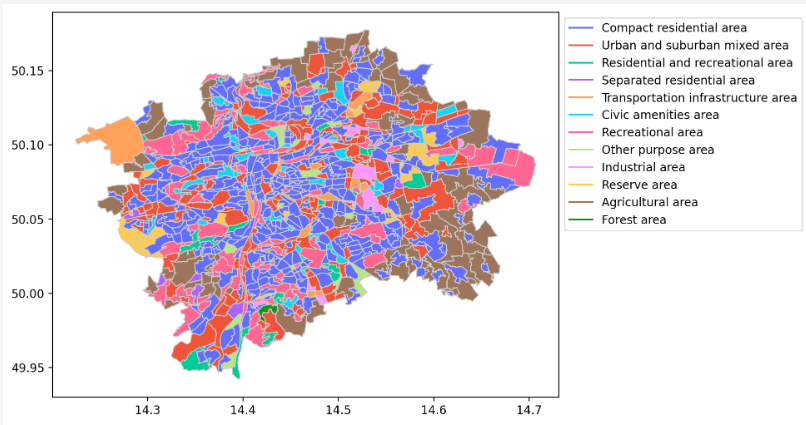
\includegraphics{zsj-type.png}
    % \caption[Problem modelling overview]{Chapter content overview. }
\end{figure}

\section{Points of Interest}


\section{People Mobility}

\begin{figure*}[hb]
    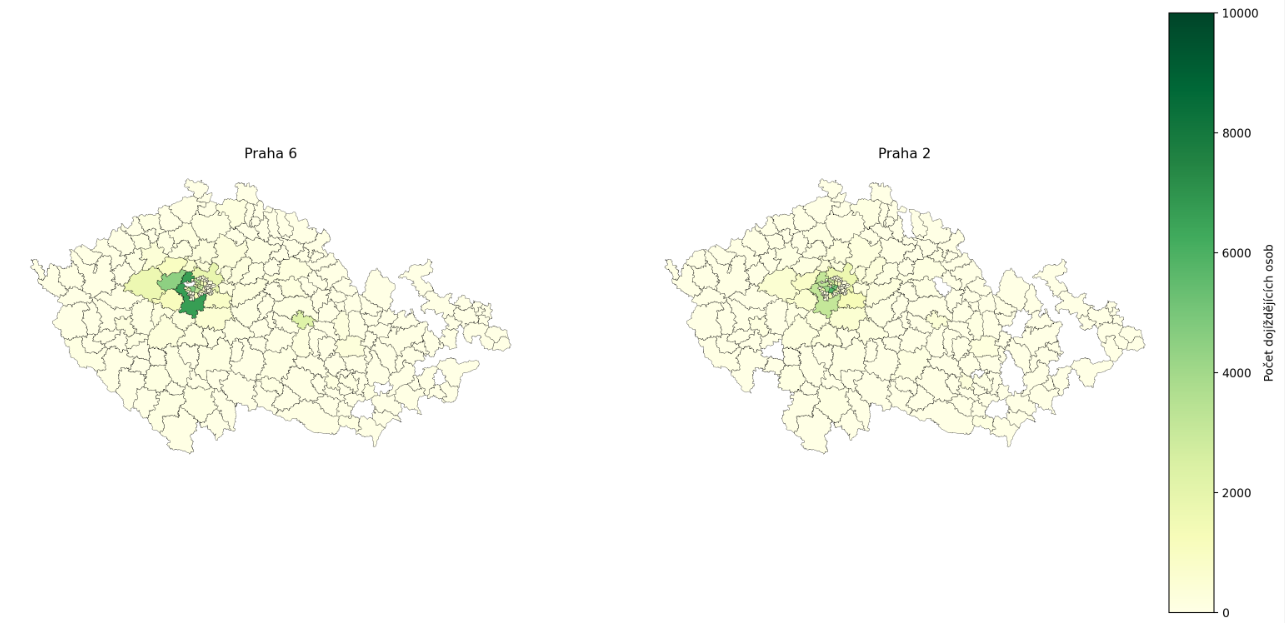
\includegraphics{commuting-people.png}
    \caption[Problem modelling overview]{Chapter content overview. }
\end{figure*}

\section{Mobility Survey - cesko v pohybu}

\begin{figure*}[hb]
    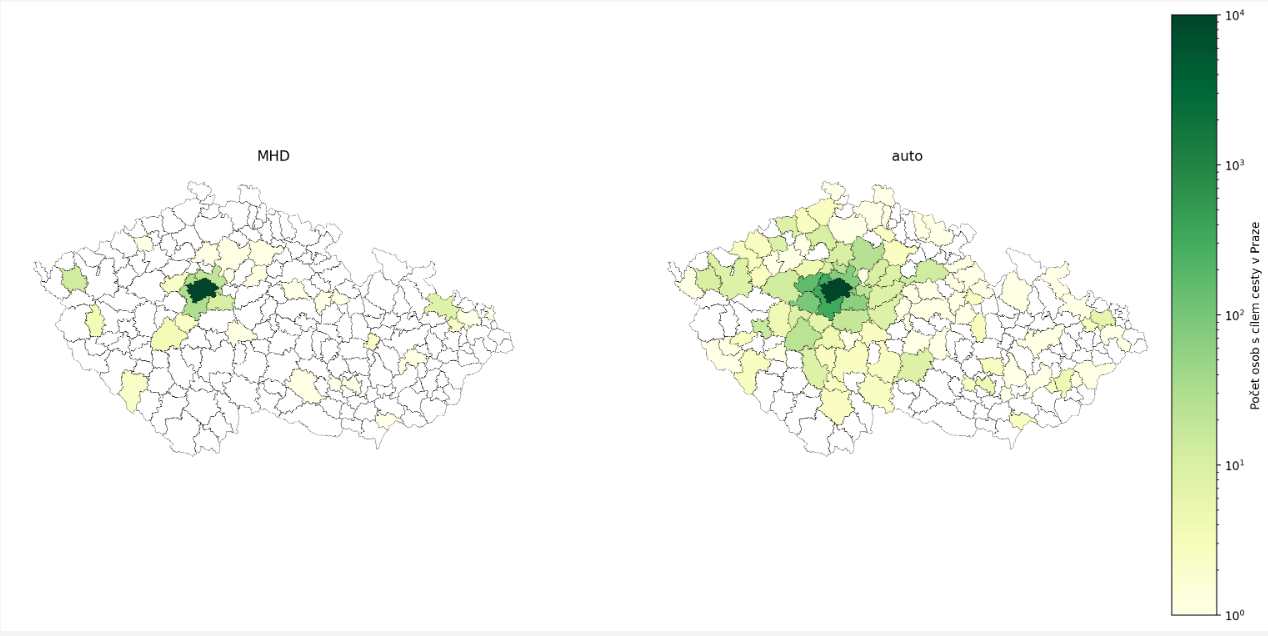
\includegraphics{vpohybu-trasnport-type.png}
    \caption[Problem modelling overview]{Chapter content overview. }
\end{figure*}

\setchapterstyle{kao}
% \setchapterpreamble[u]{\margintoc}
\chapter{Problem Modelling}
\label{ch:problem}

\begin{figure*}[hb]
    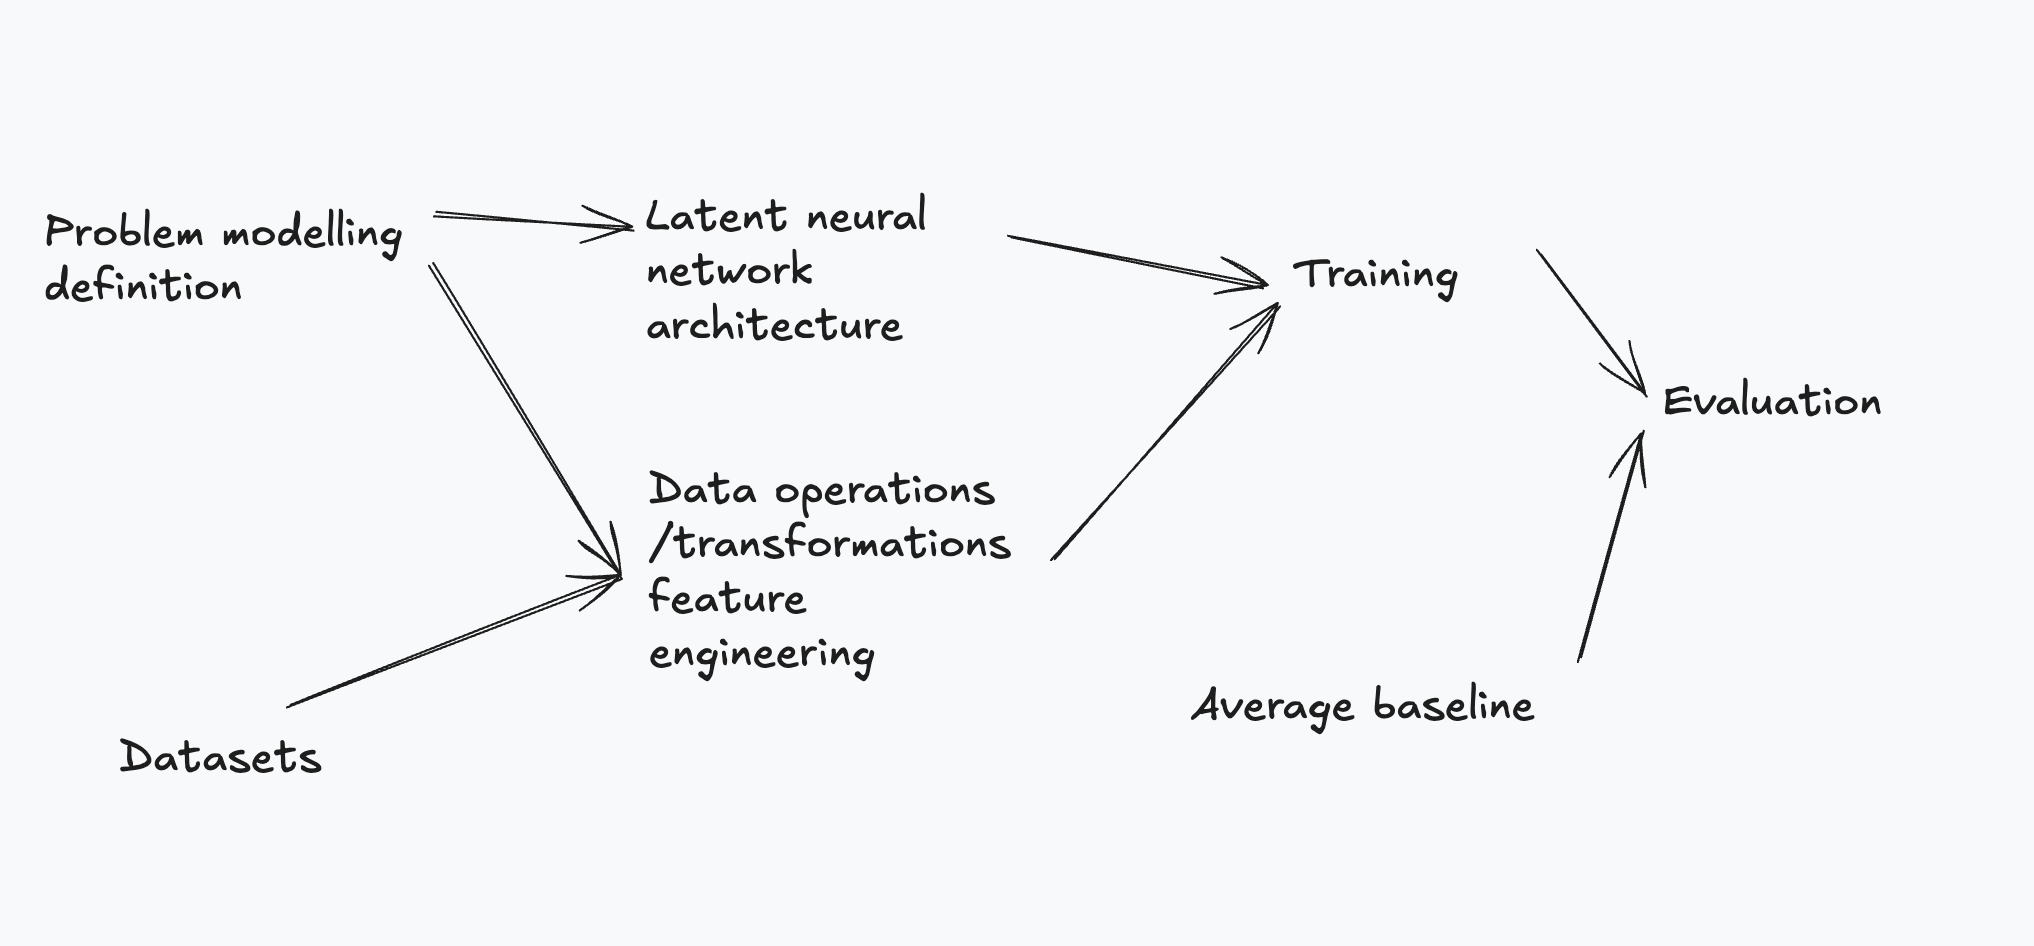
\includegraphics[width=1.5\textwidth]{diagram}
    \caption[Problem modelling overview]{Chapter content overview. }
\end{figure*}

The issue introduced in \ref{ch:problem}


\section{Problem Formulation}

Given existing sessions data and data landscape from \autoref{ch:data}. Predicting power demand for various factors for any location in prague as mentioned in \autoref{ch:problem}. Utilizing existing data. So machine learning plus addition of some more insight.

So we are interested in predicting average profile for given charger given some temporal characteristic. Like month or day of the week.


\section{Latent Nerual Network Architecture}

\todo{mention relevant literature for the latent network from literatrue research}

\begin{figure}[hb]
    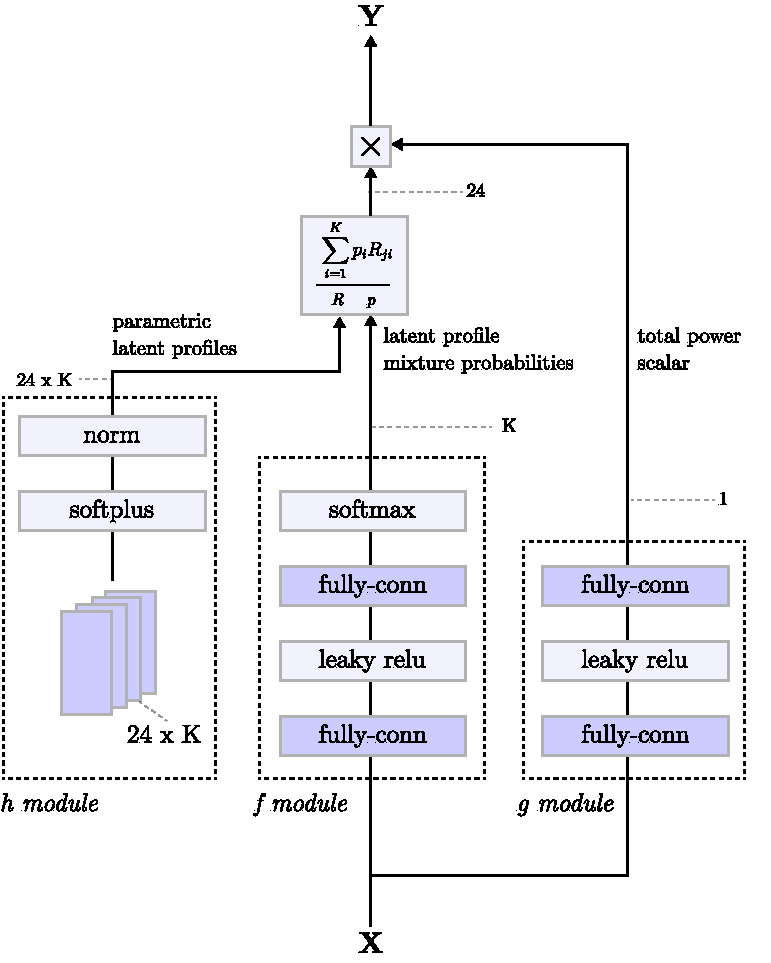
\includegraphics[width=0.7\textwidth]{nn-latent-architecture.pdf}
    \caption[Latent Neural Network Architecture]{Latent neural network architecture. Light blue rectangles denote NN layers without trainable parameters. While blue denotes layers with parameters learned by SGD. }
    \label{fig:nn-latent}
\end{figure}



\todo{mentions operations done to the data plus anaylsis of statistical impact of features on result}

\section{Training}

\todo{train test split, mention to be sure that we are learning on unseen data. So mby how there are multple chargers for one point}

\section{Baseline}

To be able to tell if our results have some value.
Are we better than average ? Because noone has done it for prague and even our greenfield problem formulation.

\setchapterstyle{kao}
\setchapterpreamble[u]{\margintoc}
\chapter{Feature Engineering}

Talks about what was extracted from datasets in \ref{ch:data}

\section{Spatial data}

\subsection{ZSJ Type and Population}

\subsection{Points of Interest}

Has statistically significant results for certain PoI \cite{hechtGlobalElectricVehicle2024}\cite{dongElectricVehicleCharging2019}
(\cite{dongElectricVehicleCharging2019} uses Gaussian cox model, \cite{hechtGlobalElectricVehicle2024} uses Neural networks and linear regression)

\cite{hechtGlobalElectricVehicle2024} states that radius of relevant PoIs is 2000metres. The research stated that the distance is sensible.
One solution is to just count all the PoIs in the radius but as they are more far away from the CP their relevance might decrease. The \cite{hechtGlobalElectricVehicle2024} thus uses importance factor for pair of PoI and CP.

$IF(PoI_i, CP_k) = max(r-d_{\text{sphere}}(PoI_i, CP_k),0)$


\subsubsection{Buildings (OsmPoisPbf)}


\subsubsection{Public Ammenities (OSMOX)}

how osmox works
\begin{figure}[hb]
    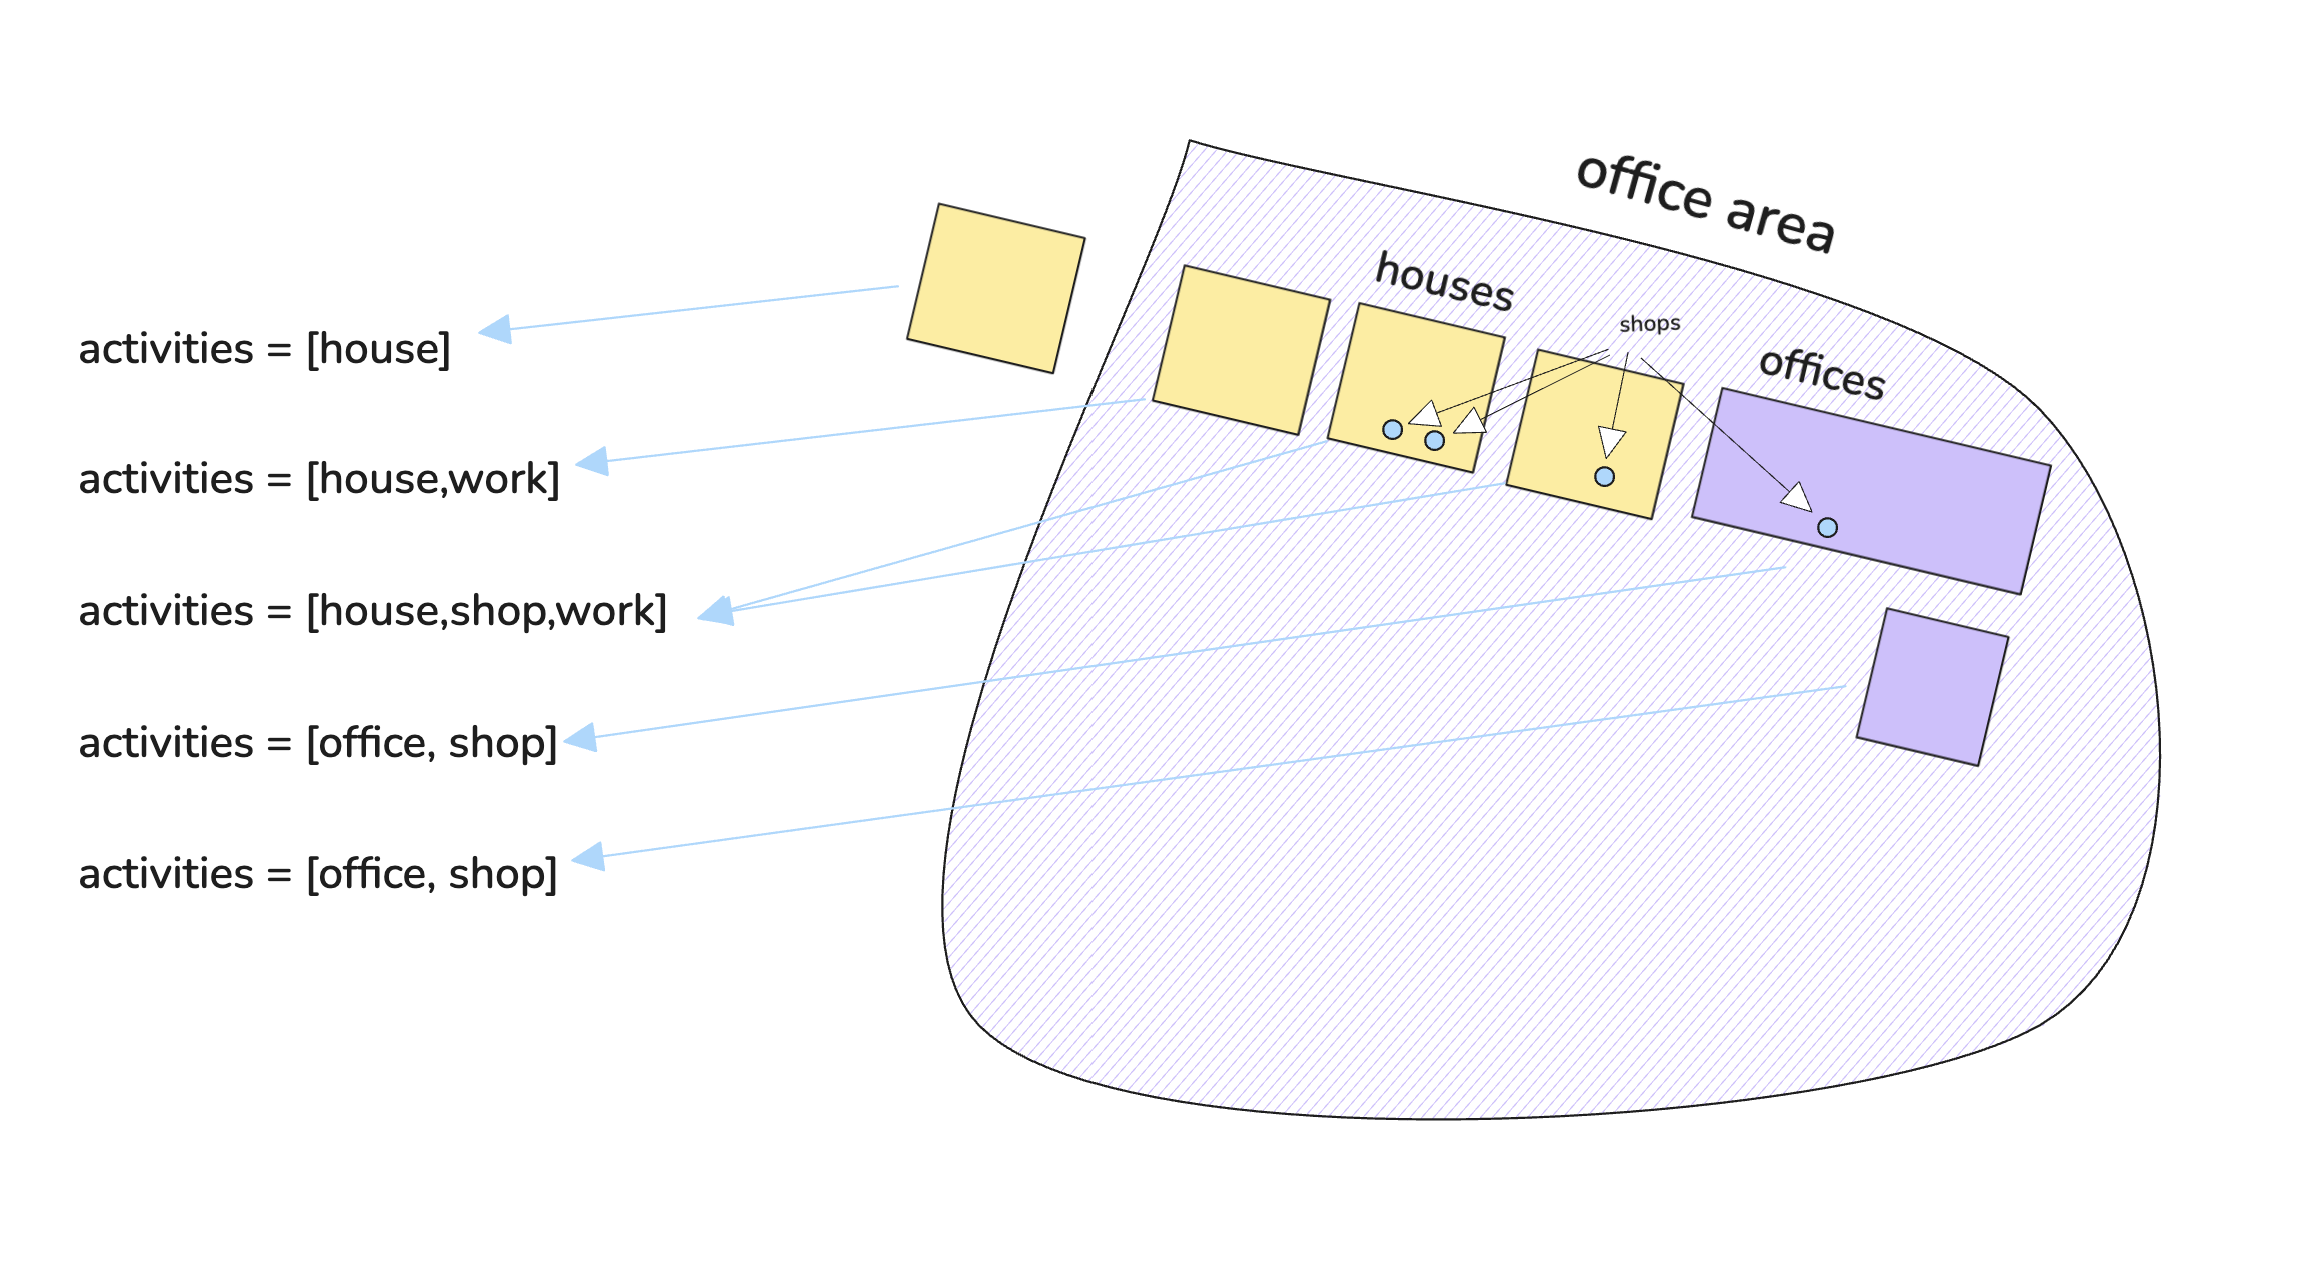
\includegraphics[width=0.7\textwidth]{osmox-poi.png}
    \caption[osmox]{osmox}
    \label{fig:nn-latent}
\end{figure}


\section{Charging profiles}


\begin{figure}[hb]
    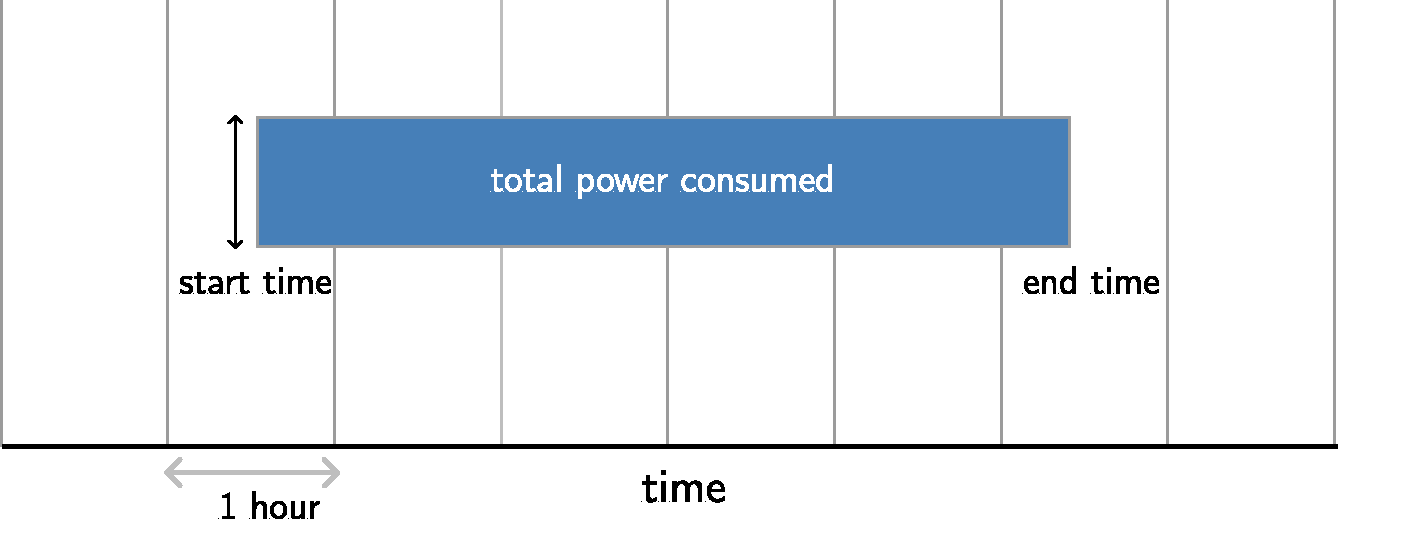
\includegraphics[width=0.7\textwidth]{cutting-1.pdf}
    % \caption[Cutting]{Cutting}
\end{figure}

\begin{figure}[hb]
    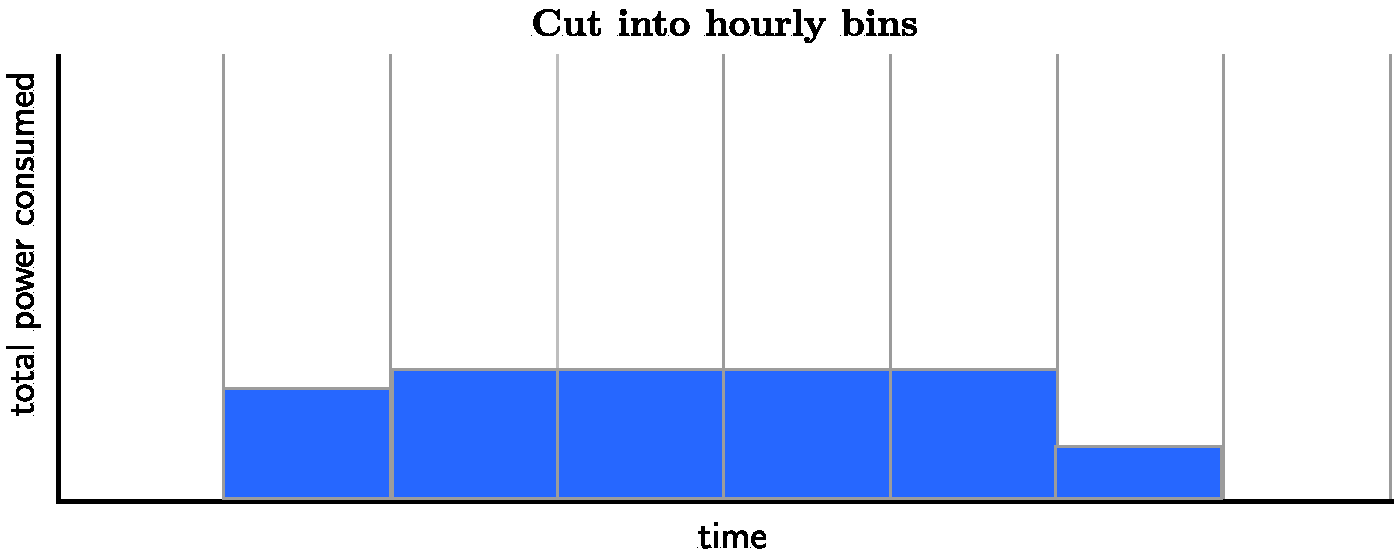
\includegraphics[width=0.7\textwidth]{cutting-2.pdf}
    % \caption[Cutting]{Cutting}
\end{figure}

\begin{figure}[hb]
    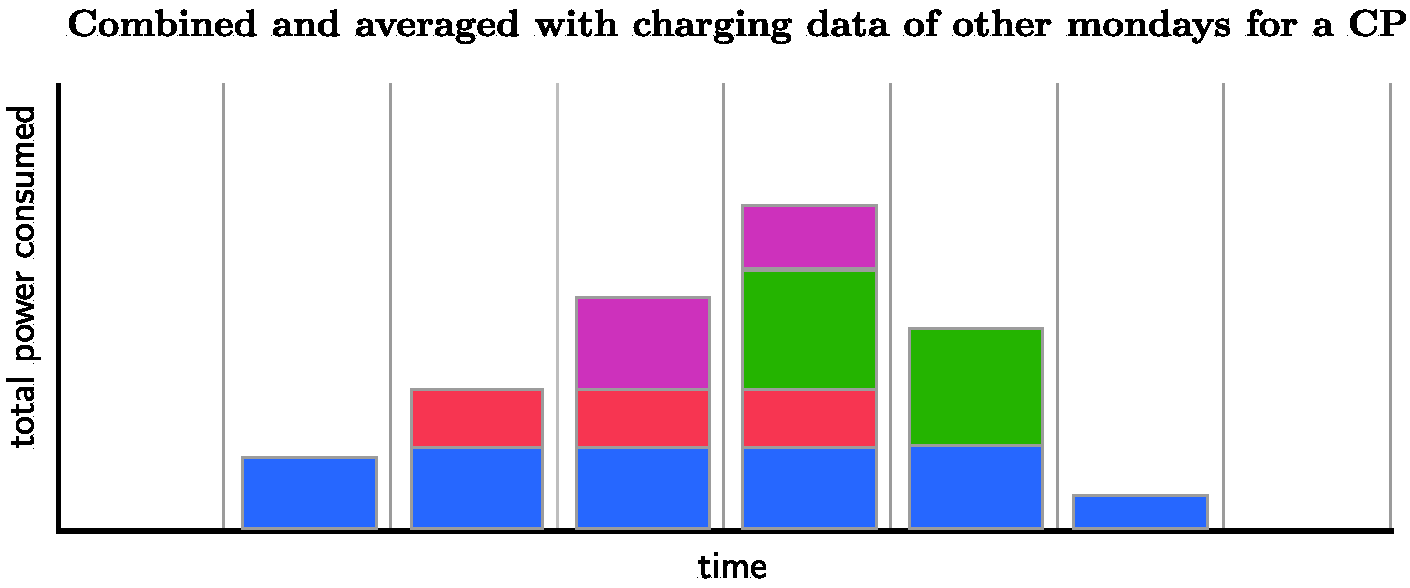
\includegraphics[width=0.7\textwidth]{cutting-3.pdf}
    % \caption[Cutting]{Cutting}
\end{figure}


\setchapterstyle{kao}
\setchapterpreamble[u]{\margintoc}
\chapter{Results}

model trained on data with results
\section{Training Results and Loss}

\section{Latent profiles interpretation}


\chapter{Conclusion}

How good we think we have been. And what did this work provide.

\section{Future work}

What to do next to improve the model. What datases to be included.